\documentclass{article}

\usepackage{amsmath}
\usepackage{amssymb}
\usepackage{amsthm}
\usepackage{graphicx}
\usepackage{color}
\usepackage{subfig}
\usepackage{float} % For [H] placement
\usepackage{mathrsfs}   % \mathscr L_2 for curly L

\usepackage{listings}
%\usepackage{algorithm}
%\usepackage{algpseudocode}
\usepackage[ruled,vlined,linesnumbered]{algorithm2e}

\usepackage{booktabs}

\usepackage[bookmarks=true,ocgcolorlinks=true,plainpages=false, breaklinks=true, bookmarksopen=true, bookmarksnumbered=true]{hyperref}
%\usepackage[bookmarks=false]{hyperref}  %hide the bookmarks bar
%\hypersetup{bookmarksopen=false}  % expand tree of bookmarks or just show first level

\hypersetup{linkcolor=blue, citecolor=magenta,urlcolor=blue} % electronic
\hypersetup{colorlinks=true}

\usepackage{siunitx}
% \sisetup{%
%   mode = math,
% %  per-mode = symbol,
% %  per-mode=repeated-symbol,
%   per-mode=reciprocal,
%   detect-all
% }
\sisetup{per-mode=reciprocal}

\usepackage[T1]{fontenc}
\usepackage{palatino}

\allowdisplaybreaks

%%BeginIpePreamble

\newcommand{\secref}[1]{\S\ref{#1}}
\newcommand{\psubref}[1]{\protect\subref{#1}}

\renewcommand{\qedsymbol}{$\blacksquare$}
\renewcommand{\vec}[1]{\ensuremath{{\boldsymbol #1}}}
\newcommand{\mat}[1]{\ensuremath{\boldsymbol{#1}}}
\newcommand{\textscript}[1]{\textnormal{\scriptsize #1}}
\newcommand{\Tr}{\textnormal{Tr}}
\newcommand{\degrees}{\ensuremath{^\circ}}
\newcommand{\degree}{\ensuremath{^\circ}}

\newcommand{\PSF}{\textnormal{PSF}}

\newcommand{\superscript}[1]{\ensuremath{^{\textrm{#1}}}}
\renewcommand{\th}[0]{\superscript{th}}
\newcommand{\st}[0]{\superscript{st}}
\newcommand{\nd}[0]{\superscript{nd}}
\newcommand{\rd}[0]{\superscript{rd}}

\newcommand{\rect}{\ensuremath{\mathrm{rect}}}

\newcommand{\pd}[2]{\frac{\partial{#1}}{\partial{#2}}}

\DeclareMathOperator*{\argmin}{arg\,min}
\DeclareMathOperator*{\argmax}{arg\,max}
\DeclareMathOperator*{\var}{var}
\DeclareMathOperator*{\diag}{diag}
\DeclareMathOperator*{\rem}{rem}
\DeclareMathOperator*{\sign}{sgn}
\DeclareMathOperator*{\supp}{supp}
\DeclareMathOperator*{\comb}{comb}
\DeclareMathOperator*{\sinc}{sinc}
\DeclareMathOperator*{\curl}{curl}
\DeclareMathOperator*{\diverge}{div}
\DeclareMathOperator*{\image}{Im}
\DeclareMathOperator*{\rank}{rank}
\DeclareMathOperator*{\range}{range}
\DeclareMathOperator*{\Real}{Re}
\DeclareMathOperator*{\Imag}{Im}

%%EndIpePreamble

\usepackage[T1]{fontenc}
\usepackage{palatino}

\usepackage{siunitx}
% \sisetup{%
%   mode = math,
% %  per-mode = symbol,
% %  per-mode=repeated-symbol,
%   per-mode=reciprocal,
%   detect-all
% }
% \sisetup{per-mode=reciprocal}

\title{PCRB}
\author{Kelvin Layton}
\date{\today}

\begin{document}

\section{Model}

The model takes the form
\begin{align}
	\vec x_k &= \vec f(\vec x_{k-1}) + \vec v_k \\
	\vec y_k &= \mat H\vec x_{k-1} + \vec w_k
\end{align}
where $\vec v_k$ and $\vec w_k$ are white, uncorrelated, zero mean Gaussian noise vectors with covariances of $\mat Q$ and $\mat R$, respectively.


\subsection{Pendulum example}

Let $\vec x_k = [a_k\quad b_k]^T$ where $a_k$ is the pendulum angle and $b_k$ is the angular velocity,
\begin{align}
	\vec f(\vec x_{k}) &= \left[\begin{array}{c}
								a_k + b_k\Delta \\ -b_k - g\sin(a_k)\Delta
								\end{array}\right]
\end{align}
The linearisation used for the EKF is
\begin{align}
	\mat F(\vec x_{k}) &= \left[\begin{array}{cc}
					1 & \Delta \\
					-g\cos(a_k) & 1 \\
				\end{array}\right]
\end{align}
The observation matrix is $H=[1\quad 0]$, so that only the first state element is measured.

\section{PCRB}

The PCRB is computed from the Fisher information matrix computed on the joint density $p(\vec y,\vec x)$,
\begin{align}
	\mat J &= \mathbb E\left[ \nabla_{\vec x}\nabla_{\vec x}^T \log p(\vec y,\vec x) \right]
\end{align}
where the expectation is taken over $\vec y$ and $\vec x$. A recursive formula was developed in \cite{Tichavsky1998} and is based on the transition density,
\begin{align}
	p(\vec x_k|\vec x_{k-1}) &= \mathcal N(\vec f(\vec x_{k-1})),\mat Q) \\
	&= (2\pi)^{-d/2} |\mat Q|^{-1/2} \exp\left(-\frac{1}{2}(\vec x_k - \vec f(\vec x_{k-1}))^T \mat Q^{-1} (\vec x_k - \vec f(\vec x_{k-1})) \right)
\end{align}
The PCRB is calculated using the logarithm of the transition density,
\begin{align}
	\log p(\vec x_k|\vec x_{k-1}) = C -\frac{1}{2}(\vec x_k - \vec f(\vec x_{k-1}))^T \mat Q^{-1} (\vec x_k - \vec f(\vec x_{k-1})) 
\end{align}
The derivatives are
\begin{align}
	\nabla_{\vec x_k}^T \log p(\vec x_k|\vec x_{k-1}) &= -(\vec x_k - \vec f(\vec x_{k-1}))^T\mat Q^{-1}  \\
	\nabla_{\vec x_k}\nabla_{\vec x_k}^T \log p(\vec x_k|\vec x_{k-1}) &= -\mat Q^{-1} \\
	\nabla_{\vec x_{k-1}}\nabla_{\vec x_k}^T \log p(\vec x_k|\vec x_{k-1}) &= \mat F(\vec x_{k-1})\mat Q^{-1} \\
	\nabla_{\vec x_{k-1}}^T \log p(\vec x_k|\vec x_{k-1}) &= (\vec x_k - \vec f(\vec x_{k-1}))^T\mat Q^{-1} \mat F(\vec x_{k-1}) \\
	\nabla_{\vec x_{k-1}}\nabla_{\vec x_{k-1}}^T \log p(\vec x_k|\vec x_{k-1}) &= -\mat F(\vec x_{k-1})^T\mat Q^{-1} \mat F(\vec x_{k-1}) 
\end{align}
Now the terms in the recursive formula for the Fisher information matrix are
\begin{align}
	 \mat U_k &= \mathbb E\left[ \mat F(\vec x_{k-1})^T\mat Q^{-1} \mat F(\vec x_{k-1}) \right ] \label{eqn:pcrb_u} \\
	\mat V_k &= \mathbb E\left[ -\mat F(\vec x_{k-1})^T\mat Q^{-1} \right ] \label{eqn:pcrb_v} \\
	\mat W_k &= \mat H^T\mat R^{-1}\mat H + \mat Q^{-1}
\end{align}

\subsection{Monte Carlo approximation}

The expectations in \eqref{eqn:pcrb_u} and \eqref{eqn:pcrb_v} can be approximated by numerical integration using many trajectory realisations. That is,
\begin{align}
	\mat U_k &\approx \frac{1}{M}\sum_{i=1}^M \mat F(\vec x_{k-1}^{(i)})^T\mat Q^{-1} \mat F(\vec x_{k-1}^{(i)}) \\
	\mat V_k &\approx \frac{1}{M}\sum_{i=1}^M \mat F(\vec x_{k-1}^{(i)})^T\mat Q^{-1} 
\end{align}


\subsection{Pendulum simulations}

\begin{figure}[H]
	\centering
	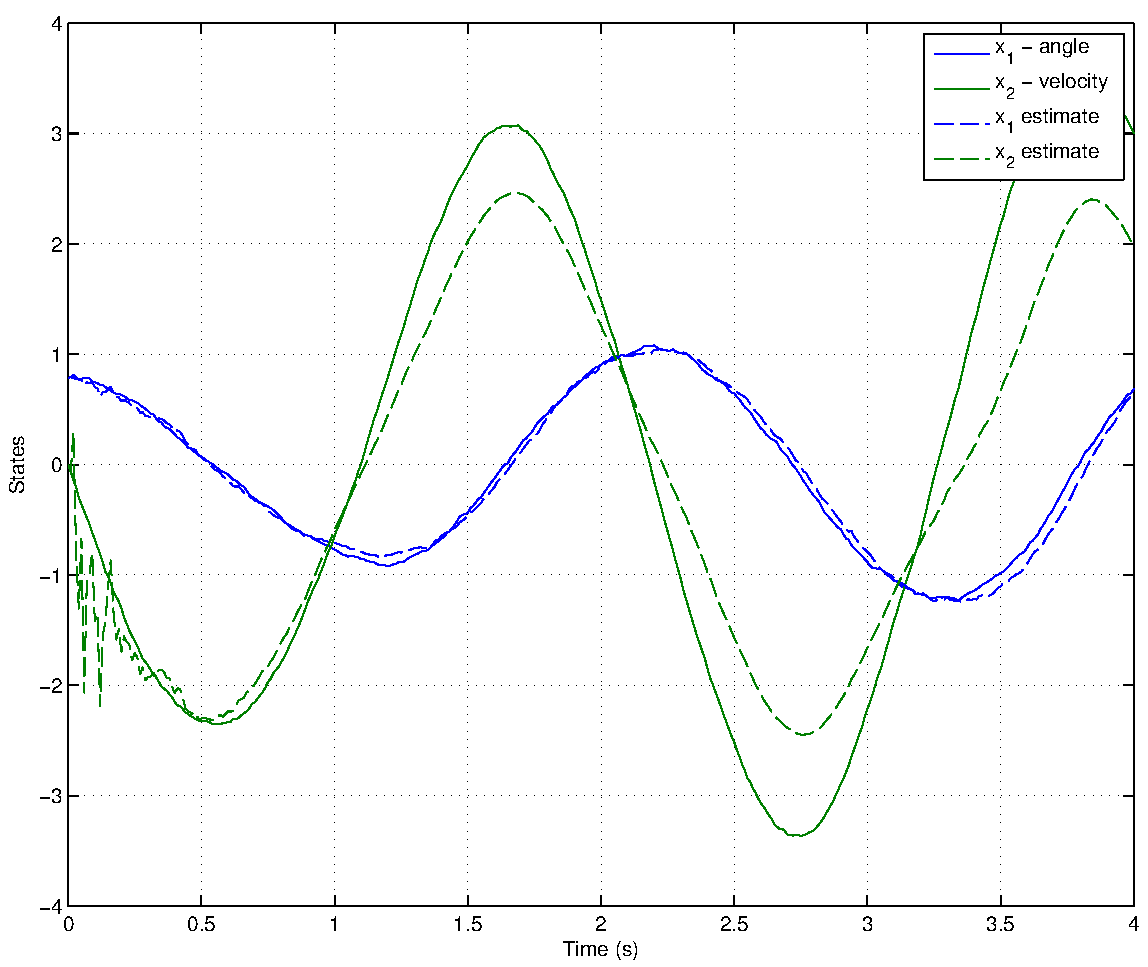
\includegraphics[width=0.75\textwidth]{figures/pendulum_trajectory}
	\caption{Trajectory of a pendulum and EKF estimates}
\end{figure}
\begin{figure}[H]
	\centering
	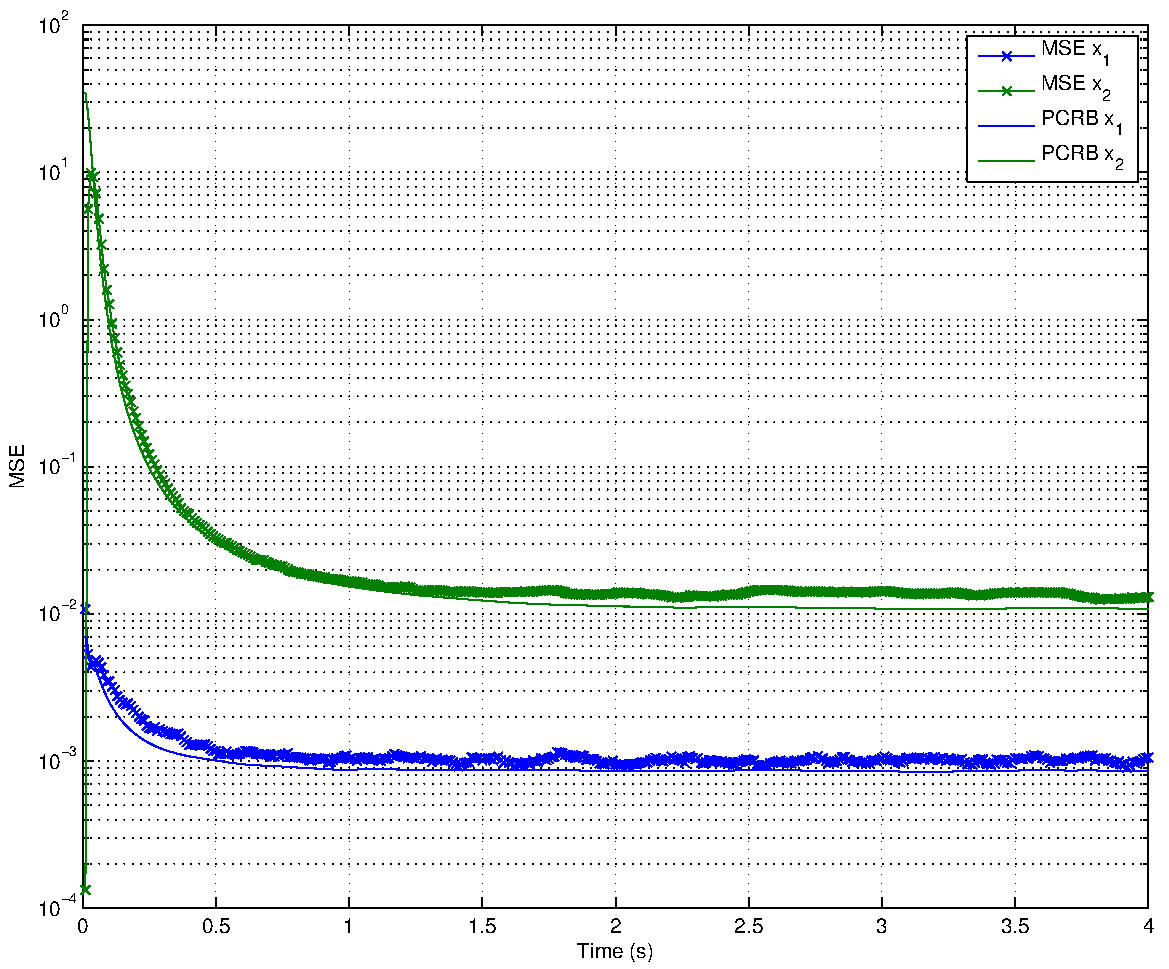
\includegraphics[width=0.75\textwidth]{figures/pendulum_pcrb}
	\caption{MSE of EKF estimates (averaged over 1000 realisations) compared to the PCRB. The suboptimal EKF is dependent on the accuracy of the linearisation at different angles, an optimal filter would achieve the CRB at all times}
\end{figure}

% \small
% \bibliographystyle{ieeetr}
% \bibliography{../library}


\end{document}
